\label{sec:empirical}
We observe several interesting phenomena which can be explained by the structural analysis of Hessian in \cref{sec:hessian}. This shows the Hessians are far from random matrices and Hessians of different models are related. This suggest more meaningful information may be extracted by assessing these common properties. We also further predict and verfy the conditions these phenomenon rely on, and thus provide some connection between network structures and Hessians. 

\subsection{Eigenspace Overlap of different models}
\label{sec:models}
Consider models trained using different random initializations with the same network structure and dataset. We observe surpisingly high top eigenspace overlap between their layerwise Hessians, despite no obvious similarity between their parameters.
%For overparameterized networks, one would expect that they should have very different parameters and thus very different layerwise Hessians. However, we observe that the top eigenspace of their layerwise Hessians have suprisingly high overlap, despite no obvious similarity between their parameters.

\begin{figure}[th]
    \centering
    \begin{subfigure}[b]{0.32\textwidth}
        \centering
        \captionsetup{justification=centering}
        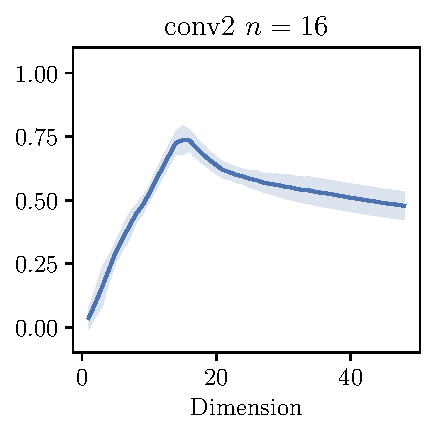
\includegraphics[width=\textwidth]{Figures/SubspaceOverlap/LeNet5_fixlr0.01/DimOverlap_CIFAR10_LeNet5_fixlr0.01_conv2.pdf}
        \caption{conv2 ($\xi = 0.027$)}
        \label{fig:Overlap_conv2}
    \end{subfigure}
    \begin{subfigure}[b]{0.32\textwidth}
        \centering
        \captionsetup{justification=centering}
        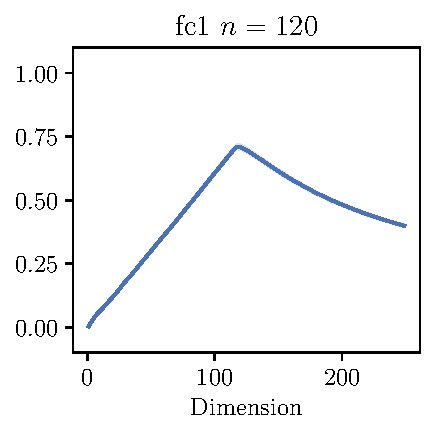
\includegraphics[width=\textwidth]{Figures/SubspaceOverlap/LeNet5_fixlr0.01/DimOverlap_CIFAR10_LeNet5_fixlr0.01_fc1.pdf}
        \caption{fc1 ($\xi =0.0047$)}
        \label{fig:Overlap_fc1}
    \end{subfigure}
    \begin{subfigure}[b]{0.32\textwidth}
        \centering
        \captionsetup{justification=centering}
        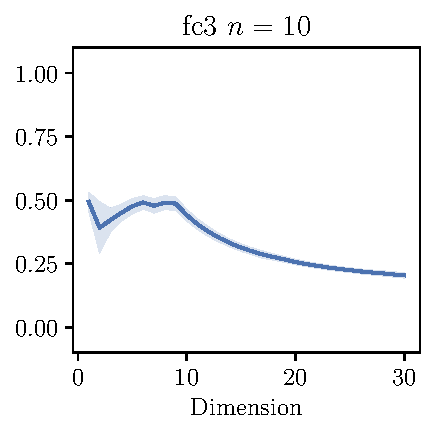
\includegraphics[width=\textwidth]{Figures/SubspaceOverlap/LeNet5_fixlr0.01/DimOverlap_CIFAR10_LeNet5_fixlr0.01_fc3.pdf}
        \caption{fc3 ($\xi =0.019$)}
        \label{fig:Overlap_fc3}
    \end{subfigure}
    \captionsetup{justification=centering}
    \caption{Eigenspace overlap between models}
    \label{fig:overlap}
\end{figure}

\cref{fig:overlap} shows the pairwise top eigenspace overlap between layerwise Hessians of 6 different models trained on CIFAR-10 with LeNet-5. The overlap is defined as in \cref{eqn:overlap}. We computed the average pairwise overlap (absolute value of normalized dot product) between their parameter vectors ($\xi$ in \cref{fig:overlap}). They are very low and similar to the expectation of random overlap $1/\sqrt{n}$. Also, if this is due to similarity of parameters, we should expect the overlap to stay high instead of having an obvious peak. We also cannot model them as 2 uncorrelated subspace in $\R^d$. In that case, their overlap should be $\frac{k}{d}$ at dimension $k$. Take layer fc1 as an example, the eigenvectors lives in dimension 48000 and are expected to have overlap 0.0025, but the actual overlap is around 0.75 as shown in \cref{fig:Overlap_fc1}.

This phenomenon, however, can be explained using the approximation in \cref{sec:approx_top_eig}. For simplicity, in this subsection we assume exactly $n$ top eigenvectors of layerwise Hessian are in $\Krsp(\tx)$. A more generalized model is in the Appendix.

Now suppose we have 2 different models with $\vt_{\vx1}$ and $\vt_{\vx2}$ respectively. We can approximate their top $k$ eigenspace as $\mU_k \otimes \vt_{\vx1}$ and $\mV_k \otimes \vt_{\vx2}$ respectively, for $k \leq n$. The eigenspace overlap at dimension $k$ is thus
\begin{equation}
\Overlap\left(\mU_k \otimes \vt_{\vx1}, \mV_k \otimes \vt_{\vx2}\right) =\frac{1}{k}\left\|\mV_1^T\mV_2 \otimes \vt_{\vx1}^T\vt_{\vx2}\right\|^2_F= \left(\vt_{\vx1} \cdot \vt_{\vx2}\right)^2\Overlap\left(\mU_k, \mV_k\right).
\label{eqn:model_overlap}
\end{equation}
Moreover, columns of $\mU_k$ and $\mV_k$ lives in $\R^n$, the space corresponding to the neurons. Since output neurons (channels for conv) can be permuted to give equivalent models while changing eigenvectors, we can assume that columns of $\mU_k$ and $\mV_k$ have no correlation and thus have an expected inner product of $\frac{1}{\sqrt{n}}$. Thus, $\Overlap(\mU_k, \mV_k) = \frac{k}{n}$ and the eigenspace overlap of at dimension $k$ would be approximately $\frac{k}{n}(\vt_{\vx1} \cdot \vt_{\vx2})^2$. This explains the peak at dimension $n$ and the linear growth before it. 

Note that fc3 does not have the linear growth since neurons cannot be permuted in the last layer. Also, a high peak means $(\vt_{\vx1} \cdot \vt_{\vx2})$ is large. \ynote{In addition, for the first layer, models with the same dataset would have the same $\tx$, and that would lead to an overlap close to 1 at dimension $n$. Omit since we did not show the first layer}

Then, consider the $(n+1)$th eigenvector of the first model. Since top $n$ eigenvectors span the full space $\Krsp(\vt_{\vx1})$, it will be orthogonal to this space. It will also have low overlap with $\Krsp(\vt_{\vx2})$ since $(\vt_{\vx1} \cdot \vt_{\vx2})$ is large. This explains the immediate drop in eigenspace overlap at dimension $n+1$. \ynote{May not be necessary}

\subsection{Dominating Eigenvectors of Layer-wise Hessian are Low Rank}
The structure of Hessians' eigenvectors is also important for assessing Hessian properties. Let $\vh_i$ be the $i$th eigenvector of a layerwise Hessian. Since it lives in the same space as the weight vector $\vw$ of that layer, we can define an operation $\Mat(\vh_i)$ to reshape $\vh_i$ into a matrix with the same shape as the weight matrix $\mW$. 

The rank of $\Mat(\vh_i)$ can be considered as an indicator of the complexity of the eigenvector. Consider the case that $\vh_i$ is one of the top eigenvectors ($i \leq t$). From \cref{sec:approx_top_eig}, we have $\vh_i \approx \vu_i \otimes \tx$ for some $\vu_i \in \R^n$. Thus, $\Mat(\vh_i) \approx \vu_i\tx^T$ and is approximately rank 1.
\begin{figure}[ht]
    \centering
    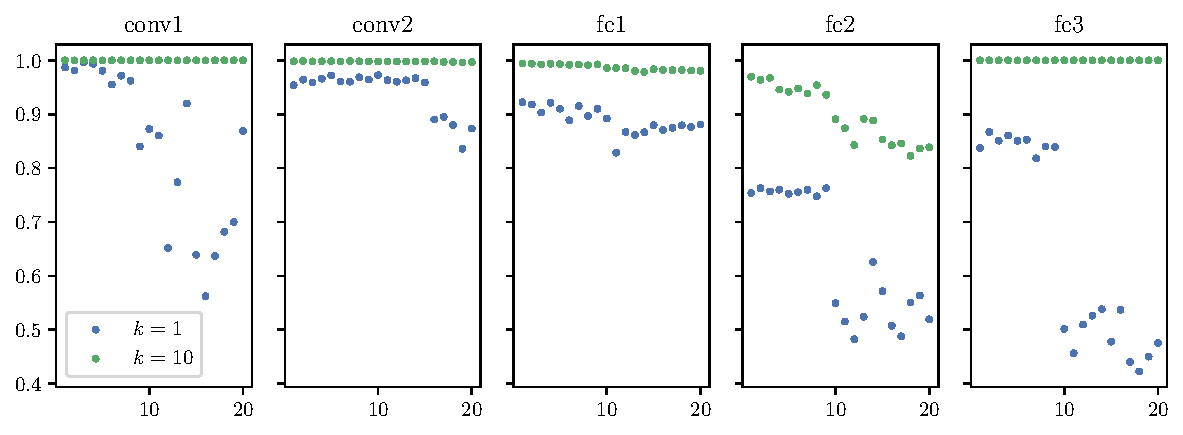
\includegraphics[width=\textwidth]{Figures/Eigenvec_Lowrank/Top_Eigenvector_rank_CIFAR10_Exp1_LeNet5_fixlr0.01R1_E-1_20_top1_10.pdf}
    \captionsetup{justification=centering}
    \caption{Ratio between spectral norm and Frobenius norm. (LeNet5 on CIFAR10)}
    \label{fig:eigen_lowrank}
\end{figure}

\cref{fig:eigen_lowrank} shows the L2 norm of top $k$ singular values divided by the Frobenius Norm of $\Mat(\vh_i)$, for $k = 1,10$. This value measures how each eigenvector is close to rank $k$. We can see the top few eigenvectors are close to rank 1. This agrees with our prediction. It also shows that the approximation is usually more accurate when $i$ is smaller.

The values are all high for $k=10$ so that all these eigenvectors can be approximated as rank 10 or lower. This results also suggest that eigenvectors of layerwise Hessians have internal structure and cannot be modelled as randomly chosen vectors in a subspace. \ynote{Can be deleted}

\subsection{Outliers in Eigenvalue Spectrum and \texorpdfstring{$\E[\mM]$}{EM}}
\label{sec:emp_outlier}
One characteristic of Hessian that has been mentioned by many is the outliers in the spectrum of eigenvalues. \citet{sagun2017empirical} suggests that there is a gap in Hessian eigenvalue distribution around the number of classes $C$ in most cases, where $C=10$ in our case. \citet{papyan2019measurements} provides further explanation for the $C$ outliers using class clustering. 

Since $\E[\vx\vx^T]$ is close to rank 1 and the Kronecker factorization is a good approximation for top eigenspace, the top eigenvalues of layerwise Hessian can be approximated as the top eigenvalues of $\E[\mM]$ multiplied by the first eigenvalue of $\E[\vx\vx^T]$. Thus, the top eigenvalues of Hessians should have the same relative ratios as the top eigenvalues of their corresponding $\E[\mM]$'s. We can also conjecture that the outliers also appear in $\E[\mM]$.

\begin{figure}[th]
    \centering
    \begin{subfigure}[b]{0.32\textwidth}
        \centering
        \captionsetup{justification=centering}
        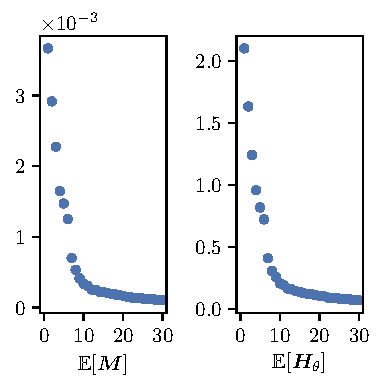
\includegraphics[width=\textwidth]{Figures/EM_vs_H/FC2_MNIST/UTAU_vs_full_sigval_d30_MNIST_Exp1_FC2_fixlr0.01R1_E-1_fc1.pdf}
        \caption{FC2 fc1 at minimum\\(MNIST)}
        \label{fig:UTAU_H_spec_FC2}
    \end{subfigure}\hfill
    \begin{subfigure}[b]{0.32\textwidth}
        \centering
        \captionsetup{justification=centering}
        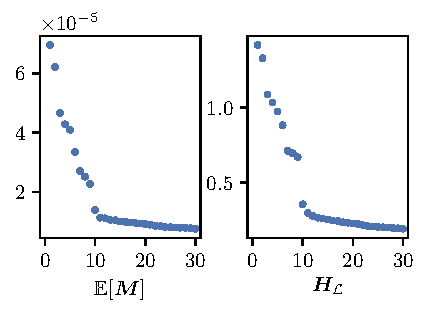
\includegraphics[width=\textwidth]{Figures/EM_vs_H/LeNet5_fixlr0.01/UTAU_vs_full_sigval_d30_CIFAR10_Exp1_LeNet5_fixlr0.01R1_E-1_fc1.pdf}
        \caption{LeNet5 fc1 at minimum\\(CIFAR10)}
        \label{fig:UTAU_H_spec_Lenet}
    \end{subfigure}\hfill
    \begin{subfigure}[b]{0.32\textwidth}
        \centering
        \captionsetup{justification=centering}
        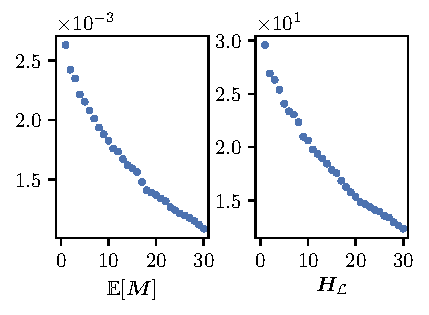
\includegraphics[width=\textwidth]{Figures/EM_vs_H/LeNet5_RL/UTAU_vs_full_sigval_d30_CIFAR10_RandomLabel_LeNet5_fixlr0.01_RLR4_E-1_fc1.pdf}
        \caption{LeNet5 fc1 at minimum\\(CIFAR10 Random Label)}
        \label{fig:UTAU_H_spec_RL}
    \end{subfigure}
    \captionsetup{justification=centering}
    \caption{Eigenspectrum of $\E[\mM]$ and $\E[\mH]$}
    \label{fig:UTAU_H_spec}
\end{figure}

Figure 7 shows the similarity of eigenvalue spectrum between $\E[\mM]$ and layerwise Hessians in different situations, agreeing with our prediction.

However, the outliers only appear at initialization and at minimum for true labels but not at miminum for random labels, contradicting to the fact that one may assume that random initialization is closer to the case of random labels. 

\citet{papyan2019measurements} provides explanation for the gap in eigenspectrum using class clustering. Although we reproduced their results on their networks, there is no clear class clustering for both $\E[M]$ and layerwise Hessian at the Minimum for networks we experiment on. The reason is unclear but we conjecture that class clustering is only significant for very large networks.

The outliers at initialization, however, are easier to explain. Similar to \citet{papyan2019measurements} suggests for full Hessian, we observe logit clustering in $\E[\mM]$'s. Since there are $C$ logits, we would expect there are $C$ outliers. The results are shown in Appendix.

\subsection{Zero-mean Batch Normalization}
\snote{The approximation worsen, but is still relevant. Reason of low overlap: low correlation between $x$ in different layers, random permutation of neurons in FC layers.}
According to our explanation, the good approximation and high overlap of top eigenspace both depend on the low rank structure of $\E[\vx\vx^T]$. Also, the low rank strcuture is caused by the fact $\E[\vx]\E[\vx]^T]$ dominates $\mSigma_\vx$ in most cases. Thus, we conjecture using Batch normalization (BN) \citep{ioffe2015batch} will change these phenomena as $\E[\vx]$ will be zero and $\E[\vx\vx^T] = \mSigma_\vx$.

We experiment on the same networks but with BN. The results are shown in the Appendix. We found that $\E[\vx\vx^T]$ is no longer close to rank 1 for models trained with BN. However, $\E[\vx\vx^T]$ still have a few large eigenvalues and is not similar to a random matrix.

In the case, our approximation in \cref{sec:approx_top_eig} is not accurate. Thus, the overlap of top $k$ eigenspace between different models can no longer be approximated as in \cref{eqn:model_overlap}. As expected, models with BN give a much lower eigenspace overlap at dimension smaller than $n$ and there is no obvious peak.

The approximation of Hessian eigenvalues using Kronecker factorization is also not so accurate in models using BN, agreeing with our conjecture. However, the approximation still gives meaningful information and the top eigenspace overlap between true and approximated hessian is still (). It is lower than the case without BN but much larger than the expected value for 2 random subspaces.